% MiniDB 实验二（索引）实验报告
% 编译：xelatex report-exp2.tex（运行两次以生成目录）
\documentclass[11pt,a4paper]{ctexart}

\usepackage[margin=2.4cm]{geometry}
\usepackage{booktabs}
\usepackage{longtable}
\usepackage{tabularx}
\usepackage{array}
\usepackage{xcolor}
\usepackage{listings}
\usepackage{graphicx}
\usepackage{tikz}
\usetikzlibrary{positioning,calc,fit,decorations.pathreplacing}
\usepackage{amsmath}
\usepackage{enumitem}
\usepackage{caption}
\usepackage{float}
\usepackage{fancyhdr}
\usepackage[hidelinks]{hyperref}

\setlist{itemsep=2pt,topsep=4pt}
\setlength{\emergencystretch}{3em}
\captionsetup{font=small,labelfont=bf}
\renewcommand{\arraystretch}{1.15}

\definecolor{codebg}{RGB}{247,247,247}
\definecolor{codecomment}{RGB}{0,110,0}
\definecolor{codekw}{RGB}{0,0,160}
\definecolor{todo}{RGB}{200,0,0}

% 待填写的内容用红色标出，定稿前全部替换
\newcommand{\TODO}[1]{\textcolor{todo}{【待填写：#1】}}

\lstset{
  basicstyle=\ttfamily\footnotesize,
  backgroundcolor=\color{codebg},
  keywordstyle=\color{codekw}\bfseries,
  commentstyle=\color{codecomment},
  frame=single, rulecolor=\color{black!25},
  breaklines=true, columns=fullflexible, keepspaces=true,
  showstringspaces=false, tabsize=2,
  numbers=left, numberstyle=\tiny\color{black!50}, xleftmargin=2em,
}
\lstdefinestyle{plain}{numbers=none,xleftmargin=0pt,keywordstyle=,commentstyle=}
\lstdefinestyle{wide}{style=plain,basicstyle=\ttfamily\scriptsize}

\pagestyle{fancy}
\fancyhf{}
\fancyhead[L]{\small 数据库系统实验二：索引}
\fancyhead[R]{\small MiniDB 实验报告}
\fancyfoot[C]{\thepage}

\newcommand{\code}[1]{\texttt{#1}}

\begin{document}

% ------------------------------------------------------------------ 封面
\begin{titlepage}
  \centering
  \vspace*{3cm}
  {\Huge\bfseries 数据库系统实验报告\par}
  \vspace{1cm}
  {\LARGE 实验 02：索引\par}
  \vspace{0.6cm}
  {\large MiniDB —— 外存 B+ 树索引的建立、维护与查找\par}
  \vspace{3cm}
  \begin{tabular}{rl}
    课程名称： & 数据库系统 \\[4pt]
    小组成员： & 任勇宁，彭文博，边宇晗，章国文，张睿涵 \\[4pt]
    提交日期： & 2026 年 11 月 11 日 \\
  \end{tabular}
  \vfill
  {\small 代码仓库：\url{https://github.com/renyongning/MiniDB}\par}
\end{titlepage}

\tableofcontents
\newpage

% ================================================================== 1
\section{实验分工安排}

实验二在实验一的存储引擎之上实现索引管理器：对已有表建立外存 B+ 树索引，随增删改维护索引，并让查询利用索引定位记录。

\begin{table}[H]
  \centering
  \caption{小组分工}
  \begin{tabularx}{\textwidth}{l X}
    \toprule
    成员 & 负责内容 \\
    \midrule
    任勇宁 & \TODO{本次实验负责内容} \\
    彭文博 & \TODO{本次实验负责内容} \\
    边宇晗 & \TODO{本次实验负责内容} \\
    章国文 & \TODO{本次实验负责内容} \\
    张睿涵 & \TODO{本次实验负责内容} \\
    \bottomrule
  \end{tabularx}
\end{table}

\paragraph{工作内容与进度}
下面按代码提交顺序列出本次实验的工作项，供填写分工时对照：
\begin{itemize}
  \item B+ 树索引的第一版（PR \#3）：索引文件与页格式、插入分裂、删除借位与合并、范围扫描、\code{CREATE/DROP INDEX}、增删改维护、\code{PRAGMA} 展示、随机测试与 TPC-H 验收程序；
  \item 代码评审与改进（PR \#4）：外部归并排序批量建树、节点按页内字节操作、\code{UPDATE/DELETE} 通过索引定位、比较运算符与 PRAGMA 的结构整理、统一代码格式；
  \item 测试与证据：150 万行 orders 与 600 万行 lineitem 上的规模测试、有索引与无索引的对照测试、树结构图；
  \item 实验报告。
\end{itemize}

% ================================================================== 2
\section{实验环境}

\begin{table}[H]
  \centering
  \caption{开发与测试环境}
  \begin{tabularx}{\textwidth}{l X}
    \toprule
    项目 & 说明 \\
    \midrule
    编程语言 & C++20，与实验一相同 \\
    构建工具 & CMake $\geq$ 3.16；\code{.clang-format}（Google 风格）统一代码格式 \\
    第三方依赖 & 无。B+ 树、外部归并排序、测试断言均为自行实现 \\
    本报告数据的测试平台 & Linux x86-64：Ubuntu 24.04.4 LTS，内核 7.0，AMD EPYC 9654，GCC 12.4.0，CMake 4.3.0，Release 构建 \\
    其他平台 & 第一版索引（PR \#3）在 macOS 27（arm64，Apple clang 17.0.0）上开发并通过测试；改进后的版本只在上述 Linux 平台上实测 \\
    验收平台 & \TODO{验收时使用的操作系统与编译器版本} \\
    \bottomrule
  \end{tabularx}
\end{table}

除特别说明外，测试使用 8 KB 页和默认的 1024 帧（8 MB）缓冲池；验收程序和演示脚本使用 16 帧（128 KB）缓冲池。测试数据为课程提供的 TPC-H 数据（\code{supplier} 1 万行、\code{orders} 150 万行、\code{lineitem} 600 万行）。

代码规模：核心库、shell 与测试合计约 11700 行 C++，其中索引模块（\code{src/index}、\code{src/db/index.cpp}）与索引测试约 2200 行。

% ================================================================== 3
\section{实验设计与实现}

\subsection{设计目标}

\begin{itemize}
  \item \textbf{外存索引}：索引是磁盘文件，节点是 8 KB 的页，节点之间用页号互相引用；所有读写经过实验一的缓冲池，树远大于缓冲池时也能工作。
  \item \textbf{完整的维护}：建立、插入、删除、更新、等值与范围查找，支持重复键。
  \item \textbf{两类数据类型}：整型（\code{INTEGER}、\code{BIGINT}）和字符型（\code{CHAR}、\code{VARCHAR}）。
  \item \textbf{与存储层集成}：SQL 层的 \code{INSERT}、\code{COPY}、\code{UPDATE}、\code{DELETE} 自动维护索引，\code{SELECT}、\code{UPDATE}、\code{DELETE} 的条件列有索引时自动使用。
  \item \textbf{可观察}：能图形化展示树结构，能校验整棵树的不变量。
\end{itemize}

实验要求在 B+ 树、可扩展 Hash、线性 Hash 中至少实现一种。我们选择 B+ 树，因为它同时支持等值和范围查询，叶子链上的顺序扫描也便于展示。

\subsection{总体结构}

\begin{table}[H]
  \centering
  \caption{索引相关模块}
  \begin{tabularx}{\textwidth}{l X}
    \toprule
    模块 & 职责 \\
    \midrule
    \code{src/index/bplus\_tree.*} & B+ 树本身：索引文件、节点页格式、查找、插入、删除、范围扫描、批量建树、结构校验和绘图。只依赖缓冲池和磁盘管理器，不知道 SQL 和表 \\
    \code{src/db/index.cpp} & 索引与数据库的衔接：\code{CREATE/DROP INDEX}、打开数据库时发现并加载索引、增删改后的索引维护 \\
    \code{src/db/database.cpp} & 执行器：\code{FindRows} 统一决定用索引还是堆扫描来定位行 \\
    \code{src/db/pragma.cpp} & \code{PRAGMA indexes / index\_check / index\_tree / index\_dot / index\_sort\_memory} \\
    \bottomrule
  \end{tabularx}
\end{table}

每个索引是数据库目录下 \code{indexes/} 中的一个 \code{.idx} 文件。文件名由索引名的十六进制编码得到，因此带引号的标识符里即使有斜杠也不会被当成路径。打开数据库时扫描该目录，逐个打开索引并核对它记录的表 ID、列序号、类型和长度与系统目录一致。

\subsection{索引文件与页格式}

索引文件复用实验一的文件头（第 0 页）、32 字节通用页头、CRC32C 校验和以及按区（64 页）扩展的方式，新增一种文件类型和四种页类型。

\begin{table}[H]
  \centering
  \caption{索引文件的页}
  \begin{tabularx}{\textwidth}{l l X}
    \toprule
    页号 & 页类型 & 内容 \\
    \midrule
    0 & 文件头 & 与数据文件相同，文件类型为 \code{kIndex} \\
    1 & \code{kBtreeMeta} & 索引元数据：格式版本、列序号、键类型与长度、根页号、下一个未用页号、空闲页链表头、索引项总数、索引名与表名 \\
    2 起 & \code{kBtreeLeaf} / \code{kBtreeInternal} & 树节点 \\
    2 起 & \code{kBtreeFree} & 合并后释放的页，页内存放下一个空闲页号，构成链表 \\
    \bottomrule
  \end{tabularx}
\end{table}

节点页在通用页头之后是 32 字节的节点头，然后是定长的槽位（图~\ref{fig:node}）。

\begin{figure}[H]
  \centering
  \begin{tikzpicture}[font=\small, box/.style={draw, minimum height=0.8cm, inner sep=2pt}]
    \node[box, minimum width=2.2cm, fill=black!8] (h) {通用页头};
    \node[box, minimum width=1.3cm, right=0pt of h] (c) {项数};
    \node[box, minimum width=1.8cm, right=0pt of c] (n) {下一叶};
    \node[box, minimum width=2.0cm, right=0pt of n] (f) {最左孩子};
    \node[box, minimum width=1.2cm, right=0pt of f, fill=black!4] (r) {保留};
    \node[box, minimum width=2.6cm, right=0pt of r, fill=blue!8] (s0) {槽位 0};
    \node[box, minimum width=2.6cm, right=0pt of s0, fill=blue!8] (s1) {槽位 1};
    \node[box, minimum width=1.2cm, right=0pt of s1] (d) {$\cdots$};
    \node[below=2pt of h] {0--31};
    \node[below=2pt of c] {32};
    \node[below=2pt of n] {36};
    \node[below=2pt of f] {40};
    \node[below=2pt of s0] {64};
    \node[box, minimum width=3.4cm, below=1.5cm of n, fill=blue!8] (k) {键};
    \node[box, minimum width=2.4cm, right=0pt of k, fill=blue!8] (rid) {RID（6 字节）};
    \node[box, minimum width=3.4cm, right=0pt of rid, fill=blue!8] (ch) {右孩子页号（4 字节）};
    \draw[dashed] (s0.south west) -- (k.north west);
    \draw[dashed] (s0.south east) -- (ch.north east);
    \node[below=2pt of k] {整型 8 字节；字符型 $2+n$ 字节};
    \node[below=2pt of ch] {仅内部节点};
  \end{tikzpicture}
  \caption{节点页布局。槽位定长，叶子的槽位是（键，RID），内部节点的槽位多一个右孩子页号}
  \label{fig:node}
\end{figure}

\begin{itemize}
  \item 整型键统一存成 8 字节有符号整数；字符型键存 2 字节长度加内容，槽位宽度按列的声明长度 $n$ 固定。
  \item 内部节点的第 $i$ 个槽位存放第 $i$ 个分隔键和它右边的孩子，最左边的孩子存在节点头里。这样在内部节点插入“一个分隔键和它右边的新孩子”正好是插入一个槽位，合并时删除“一个分隔键和它右边的孩子”正好是删除一个槽位。
  \item 节点容量（最大项数）为 $\lfloor (8192-64)/(\text{键宽}+6+4) \rfloor$ 向下取偶，叶子和内部节点共用。整型键为 450，\code{CHAR(25)} 为 218，\code{CHAR(15)} 为 300。非根节点至少半满。
\end{itemize}

\subsection{键的顺序与重复键}

索引是非唯一的。为了让重复键也有确定的顺序，树里的每一项按 \textbf{（键，RID）} 排序：键相同的项按记录地址排序。这样做有三个好处：重复键可以跨越多个叶子而不需要溢出页；删除时能精确定位到要删的那一项，不必在一串相同的键里线性查找；内部节点的分隔键也是（键，RID），子树的键范围没有歧义。

键的比较与 SQL 层保持一致：整数直接按 64 位整数比较（超过 $2^{53}$ 的相邻值也能区分）；字符串按字节的字典序比较，并且尾部空白不参与比较，所以 \code{CHAR(n)} 列补齐的空格不影响与字面量的匹配。\code{NULL} 不进入索引，因为它不满足任何比较条件。

\subsection{查找与范围扫描}

点定位从根开始，每层在节点内二分找到要进入的孩子（分隔键等于目标时走右边），直到叶子。叶子之间用“下一叶”页号串成链表，范围扫描沿链表前进。

\code{Scan(op, key, visitor)} 支持六种比较运算。有下界的运算（$=$、$>$、$\geq$）先定位到键所在的叶子再向右扫描；没有下界的（$<$、$\leq$、$\neq$）从最左叶子开始。有上界的运算（$=$、$<$、$\leq$）在遇到第一个超过键的项时停止。访问函数返回 \code{false} 可以提前结束，\code{LIMIT} 由此实现。

\subsection{插入与分裂}

插入自顶向下递归到叶子，在叶子内二分找到位置并插入。如果节点的项数超过容量，就把上半部分移到新分配的右兄弟：
\begin{itemize}
  \item 叶子分裂时，中间项留在右兄弟里并复制一份作为分隔键交给父节点，同时把右兄弟接入叶子链；
  \item 内部节点分裂时，中间的分隔键上移到父节点，不保留在任何一侧。
\end{itemize}
分裂沿递归返回路径向上传播，传到根时新建一个内部节点作为新根，树高加一。没有发生分裂的祖先节点不会被写回。

\subsection{删除、借位与合并}

删除先按（键，RID）定位并从叶子移除。如果节点因此少于半满，由父节点调整：
\begin{enumerate}
  \item 左兄弟有富余时，从左兄弟借最后一项；
  \item 否则右兄弟有富余时，从右兄弟借第一项；
  \item 都不能借时，与一个兄弟合并，父节点删除对应的分隔键和孩子，被合并掉的页进入空闲页链表。
\end{enumerate}
叶子借位后更新父节点的分隔键；内部节点借位时分隔键经过父节点“旋转”。合并可能使父节点也不足半满，调整沿路径向上传播。内部根节点只剩一个孩子时，由这个孩子接任根，树高减一。只有发生变化的节点才写回：没有触发调整的祖先不会被写。

空闲页链表的头在元数据页里，分配新页时优先复用空闲页，没有空闲页时才使用文件末尾的新页，文件满时按区扩展。

\subsection{内外存数据交换}

树的所有页都通过实验一的 \code{BufferPool} 读写：读取时 \code{FetchRead} 把页从磁盘调入缓冲帧并校验 CRC，写入时在缓冲帧里修改并标记为脏页，由 CLOCK 淘汰或 \code{flush} 写回磁盘。索引代码里没有任何直接的文件读写（批量建树的临时排序文件除外，见下节）。

\paragraph{节点的工作副本}
树的操作需要同时看到多个节点：分裂涉及节点和新兄弟，借位与合并涉及父节点、当前节点和兄弟。如果每个节点都钉住一个缓冲帧，小缓冲池下会出现无帧可用的情况。因此 \code{Node} 是一页的\textbf{工作副本}：读节点时把页的字节复制出来并立即释放缓冲帧，修改在副本上进行，写节点时再申请缓冲帧把字节复制回去。这样树在任何时刻最多只占用一个缓冲帧，测试中用 2 帧的缓冲池也能完成深度超过 5 层的树的全部操作。范围扫描时叶子同样是副本，访问函数里回表读堆页不会与索引页争用缓冲帧。

\paragraph{按页内字节操作}
工作副本保持页的磁盘编码，不解码成对象：查找直接比较槽位里的字节，插入和删除是一次 \code{memmove}，分裂与合并是整段槽位的复制。只有在需要把某一项交给调用者时（分隔键、扫描结果、绘图）才解码那一项。第一版实现每访问一个节点都把整页解码成“值对象”的数组、写回时再重新编码，性能分析显示这部分占插入 CPU 时间的七成左右；改为按字节操作后，磁盘格式完全不变，新旧程序可以互相读写对方的索引文件。

\subsection{建立索引：外部归并排序与自底向上装载}

对已有数据的表建索引时，逐条插入是最直接的做法，但每条都要从根走到叶，而且按键的顺序插入会使每个叶子在分裂后只有半满。我们采用数据库系统通用的做法（PostgreSQL、InnoDB 建 B 树索引都是这一思路）：先把所有（键，RID）排序，再从叶子层开始顺序地把树写出来。排序使用外部归并，因此建索引所需的内存有上限，与表的大小无关。

\begin{enumerate}
  \item \textbf{生成有序段}：扫描堆表，把每行的（键，RID）编码成紧凑的记录追加到一块固定大小的排序缓冲里（默认 64 MB，可用 \code{PRAGMA index\_sort\_memory} 调整）。缓冲一次分配、不再增长；下一条记录放不下时，对缓冲排序并把它作为一个\textbf{有序段}追加到临时文件，然后清空缓冲继续。
  \item \textbf{多路归并}：全部读完后，用小顶堆对各个有序段做多路归并，每个段只在内存里保留一个读缓冲（排序预算的八分之一，限制在 8 KB 到 64 KB 之间）。预算能负担的读缓冲数就是归并的路数；有序段比这更多时，先把相邻的若干段归并成更长的段（一趟归并），重复到一次归并能完成为止。
  \item \textbf{自底向上装载}：归并输出的有序流直接填充叶子页，页满即写出，并把它的页号和最小项交给上一层；上一层以同样的方式填充。每一层在内存里只有一个正在填充的节点。
\end{enumerate}

两点细节：
\begin{itemize}
  \item 装载时每个节点预留八分之一的空间，使建好之后的头几次插入不会立即引起分裂。
  \item 我们的树要求非根节点至少半满，而简单地“填满一页写一页”会让每层的最后一页可能不足半满。由于归并前已经知道总项数，每一层有多少个节点、每个节点放多少项都可以预先算好并均匀分配，所以流式装载仍然能保证不变量。
\end{itemize}

数据在排序缓冲里放得下时不产生临时文件，直接在内存排序后装载。\code{CREATE INDEX} 的结果消息会说明走的是哪条路径，例如 \code{sorted in memory} 或 \code{external sort: 1710 runs merged in 4 passes}。建树写入的是一个 \code{.building} 临时文件，全部完成并刷盘后才改名为 \code{.idx}，所以打开数据库时不会看到建到一半的索引。

\subsection{与 SQL 层的衔接}

\paragraph{用索引定位行}
\code{SELECT}、\code{UPDATE}、\code{DELETE} 的 \code{WHERE} 子句由同一个函数 \code{BindWhere} 绑定到表的列上，再由 \code{Database::FindRows} 统一定位满足条件的行：条件列上有索引时沿索引扫描并按 RID 回表，否则顺序扫描堆表。是否使用索引只在这一处决定。$\neq$ 条件几乎命中全表，逐项随机回表不如顺序扫描，所以不使用索引。使用了索引时，语句的结果消息里会显示 \code{INDEX SCAN 索引名}。

\code{UPDATE} 和 \code{DELETE} 先收集全部命中的行再修改。这对走索引的情形尤其必要：如果一边沿索引扫描一边修改被索引的列，被改过的项会移动到扫描尚未到达的位置而被再次命中。

\paragraph{索引维护}
\code{INSERT} 和 \code{COPY} 在堆表插入成功后把新行的键和 RID 插入该表的每个索引；\code{DELETE} 删除对应的项；\code{UPDATE} 只对键值确实发生变化的索引做一次删除和一次插入。实验一的堆表在行变长搬家时使用转发指针，行的 RID 保持不变，所以更新不改变索引列时索引完全不用动。\code{DROP TABLE} 会一并删除该表的索引。

\subsection{模块接口}

\begin{lstlisting}[language=C++,style=plain]
class BPlusTree {
 public:
  static Result<std::unique_ptr<BPlusTree>> Create(
      BufferPool& pool, const std::string& path, const IndexMetadata& metadata);
  static Result<std::unique_ptr<BPlusTree>> Open(BufferPool& pool,
                                                 const std::string& path);

  // Builds an empty tree from entries added in any order (CREATE INDEX).
  class BulkLoader {
   public:
    explicit BulkLoader(BPlusTree& tree,
                        size_t memory_bytes = kDefaultSortMemory);
    Status Add(const Value& key, RID rid);  // NULL keys are skipped
    Status Finish();
    size_t runs() const;          // sorted runs written to disk
    size_t merge_passes() const;  // extra passes when runs exceed the fan-in
  };

  Status Insert(const Value& key, RID rid);
  Status Erase(const Value& key, RID rid);
  // Visits matching entries in key order; the visitor returns false to stop
  // early (LIMIT).
  Status Scan(CompareOp op, const Value& key,
              const std::function<bool(const IndexEntry&)>& visitor);
  Result<std::vector<RID>> Find(const Value& key);

  Result<IndexStats> Validate();  // checks every invariant of the whole tree
  Result<std::string> Draw(size_t max_nodes = 128);  // indented text
  Result<std::string> Dot(size_t max_nodes = 128);   // Graphviz source
};
\end{lstlisting}

接口的设计考虑：
\begin{itemize}
  \item 树只认识“键”和“RID”，不依赖表、元组和 SQL，可以单独测试；数据地址就是实验一堆表的 RID（页号加槽号）。
  \item 所有可能失败的操作返回 \code{Status} 或 \code{Result<T>}，与存储层一致；磁盘上读到的内容（元数据、页类型、项数、页号范围）都经过检查，不一致时返回 \code{kCorruption}。
  \item \code{Scan} 用访问函数而不是一次返回全部结果，范围查询不需要把结果集物化，也使 \code{LIMIT} 可以提前终止。
  \item \code{Validate} 是面向测试和演示的：它遍历整棵树，检查键有序、分隔键范围、半满约束、叶子深度一致、叶子链完整、项数与元数据一致、空闲页链表无环且与在用页不重叠、没有不可达的页。
\end{itemize}

% ================================================================== 4
\section{使用手册}

\subsection{编译与启动}

\begin{lstlisting}[language=bash,style=plain]
cmake -S . -B build -DCMAKE_BUILD_TYPE=Release
cmake --build build -j
./build/minidb_shell --db /tmp/demo_db            # 交互式
./build/minidb_shell --db /tmp/demo_db --buffer 16 --file scripts/demo_index.txt
\end{lstlisting}

\subsection{索引相关的 SQL}

\begin{lstlisting}[language=SQL,style=plain]
CREATE INDEX [IF NOT EXISTS] index_name ON table_name(column);
DROP INDEX [IF EXISTS] index_name;

-- WHERE 列上有索引时自动使用，结果消息显示 INDEX SCAN index_name
SELECT ... FROM t WHERE column = | < | <= | > | >= value [LIMIT n];
UPDATE t SET ... WHERE column op value;
DELETE FROM t WHERE column op value;
\end{lstlisting}

索引为单列、非唯一索引，列类型可以是 \code{INTEGER}、\code{BIGINT}、\code{CHAR(n)}、\code{VARCHAR(n)}（$n \leq 4000$）。同一个表可以建多个索引。

\subsection{查看与校验}

\begin{table}[H]
  \centering
  \caption{索引相关的 PRAGMA}
  \begin{tabularx}{\textwidth}{l X}
    \toprule
    命令 & 作用 \\
    \midrule
    \code{PRAGMA indexes[(table)]} & 列出索引：所属表、列、类型、项数 \\
    \code{PRAGMA index\_check(index)} & 校验整棵树的全部不变量，并输出项数、树高、节点数、叶子数、空闲页数、节点容量、根页号（\code{index\_stats} 是它的别名） \\
    \code{PRAGMA index\_tree(index)} & 以缩进文本画出树：每个节点的页号、项数、前几个键及其 RID，叶子标出下一叶 \\
    \code{PRAGMA index\_dot(index)} & 输出 Graphviz DOT 图源，可用 \code{dot -Tsvg} 生成图片 \\
    \code{PRAGMA index\_sort\_memory [= KB]} & 查看或设置建索引的排序内存预算（当前会话有效） \\
    \code{PRAGMA buffer\_stats} & 缓冲池命中、缺页、淘汰、写回次数，用于观察内外存交换 \\
    \bottomrule
  \end{tabularx}
\end{table}

\subsection{演示与验收程序}

\begin{lstlisting}[language=bash,style=plain]
# 演示脚本：建表、导入 supplier、建两种类型的索引、画树、
# 点查与范围查、增删改、校验、小内存预算下的外部归并建树
./build/minidb_shell --db /tmp/demo_db --buffer 16 --file scripts/demo_index.txt

# 自动验收：导入 supplier，建两种索引，重开后逐条核对 20000 次点查找，
# 范围查询与全表扫描对照，增删改后再次重开核对
./build/minidb_verify_index_tpch test/tpc-h/supplier.tbl /tmp/verify_db

# 由树图文件生成报告用的结构图（需要 Graphviz）
scripts/index_figure.py supplier_key.tree supplier_key.png
\end{lstlisting}

演示脚本和验收程序都要求使用新的数据库目录。

% ================================================================== 5
\section{测试方案和结果}

\subsection{测试方案}

\begin{table}[H]
  \centering
  \caption{测试层次}
  \begin{tabularx}{\textwidth}{l X}
    \toprule
    测试 & 内容 \\
    \midrule
    树的随机测试 & 直接调用 \code{BPlusTree}：1 万个整数项和 5 千个字符串项按固定种子乱序插入、交错删除，键有大量重复；每一阶段都校验全树不变量，并把六种比较运算的扫描结果与一个独立的参考集合比对；4 帧缓冲池，跨多个区，关闭后重新打开再比对；清空后空闲页被复用 \\
    边界测试 & 容量为 2 的长字符串索引形成 5 层以上的树后全部删除回到单个根；字符串含 NUL 字节、超长键和类型不符的键被拒绝；\code{BIGINT} 的最小值、最大值和超过 $2^{53}$ 的相邻值 \\
    批量建树测试 & 三种扇出（容量 2、30、450）、多种规模（空、1、半满、刚好满、满加一、多层等），分别在内存排序和 2 KB 预算（上百个有序段、多趟归并）下建树，校验不变量并与参考集合比对，之后继续插入和删除；重复项落在不同有序段时也能发现；临时文件被清理 \\
    SQL 集成测试 & 8 帧缓冲池：建索引前后同一批查询结果一致；\code{NULL}、\code{CHAR} 补齐、\code{LIMIT}、同列多个索引、\code{COPY}、转发行；重开后索引仍可用；\code{DROP} \\
    增删改对照测试 & 同一批 16 条 \code{UPDATE/DELETE} 分别在有索引和无索引的两张相同的表上执行，每条之后比对两张表的全部内容和索引项数；包括修改被过滤的列、把键改大和改小、改为 \code{NULL}、重复键、转发行 \\
    损坏检测 & 改写索引页的一个字节后，查找返回校验和错误而不是错误结果 \\
    真实数据验收 & \code{minidb\_verify\_index\_tpch}：supplier 上两种类型的索引，重开后 2 万次点查找逐条核对 \\
    规模测试 & orders（150 万行）和 lineitem（600 万行）上建索引、查找、增删改并校验 \\
    \bottomrule
  \end{tabularx}
\end{table}

自动化测试在两种构建下运行：Release，以及开启 AddressSanitizer、UndefinedBehaviorSanitizer 和 \code{-Werror} 的构建。

\subsection{自动化测试结果}

\begin{lstlisting}[style=plain]
    Start 1: minidb_integration
1/3 Test #1: minidb_integration ...............   Passed    0.11 sec
    Start 2: minidb_storage
2/3 Test #2: minidb_storage ...................   Passed    0.02 sec
    Start 3: minidb_index
3/3 Test #3: minidb_index .....................   Passed    1.31 sec
100% tests passed, 0 tests failed out of 3
Total Test time (real) =   1.45 sec
\end{lstlisting}

\begin{lstlisting}[style=plain]
$ ./build/minidb_index_tests
integer randomized/persistence: OK
string randomized/internal splits: OK
bulk load sizes/fanouts/then maintenance: OK
tiny fanout/BIGINT boundaries: OK
SQL build/maintenance/ranges/reopen/drop: OK
UPDATE/DELETE through indexes vs. heap scan: OK
checksum corruption detection: OK
\end{lstlisting}

\subsection{supplier 上的两种索引}

在 \code{supplier}（1 万行）的 \code{s\_suppkey}（\code{INTEGER}）和 \code{s\_name}（\code{CHAR(25)}）上分别建索引，16 帧缓冲池。

\begin{table}[H]
  \centering
  \caption{supplier 两个索引的结构}
  \begin{tabular}{lrr}
    \toprule
    项目 & supplier\_key & supplier\_name \\
    \midrule
    索引列 & s\_suppkey & s\_name \\
    数据类型 & INTEGER & CHAR(25) \\
    索引项数 & 10000 & 10000 \\
    树高（根为第 1 层） & 2 & 2 \\
    节点总数 & 27 & 54 \\
    叶节点数 & 26 & 53 \\
    节点容量 & 450 & 218 \\
    结构校验 & ok & ok \\
    \bottomrule
  \end{tabular}
\end{table}

字符键更宽，每页能放的项更少，所以叶子更多。两棵树的结构见图~\ref{fig:key} 和图~\ref{fig:name}（为适应版面只画出前两个和后两个叶子，完整的树在 \code{doc/exp2-evidence/} 下的 \code{.tree} 和 \code{.dot} 文件里）。

\begin{figure}[H]
  \centering
  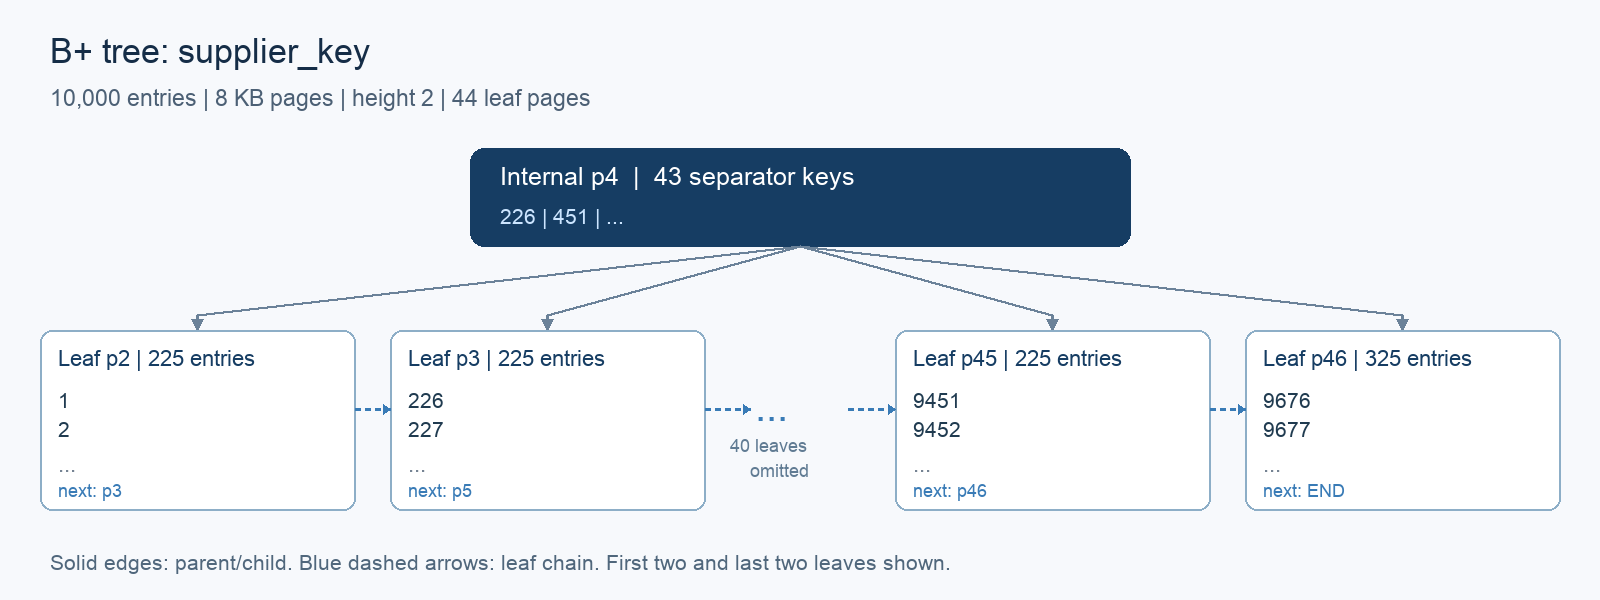
\includegraphics[width=\textwidth]{../exp2-evidence/supplier_key.png}
  \caption{supplier 整型索引的 B+ 树：根节点保存分隔键，叶子保存键与 RID 并顺序相连}
  \label{fig:key}
\end{figure}

\begin{figure}[H]
  \centering
  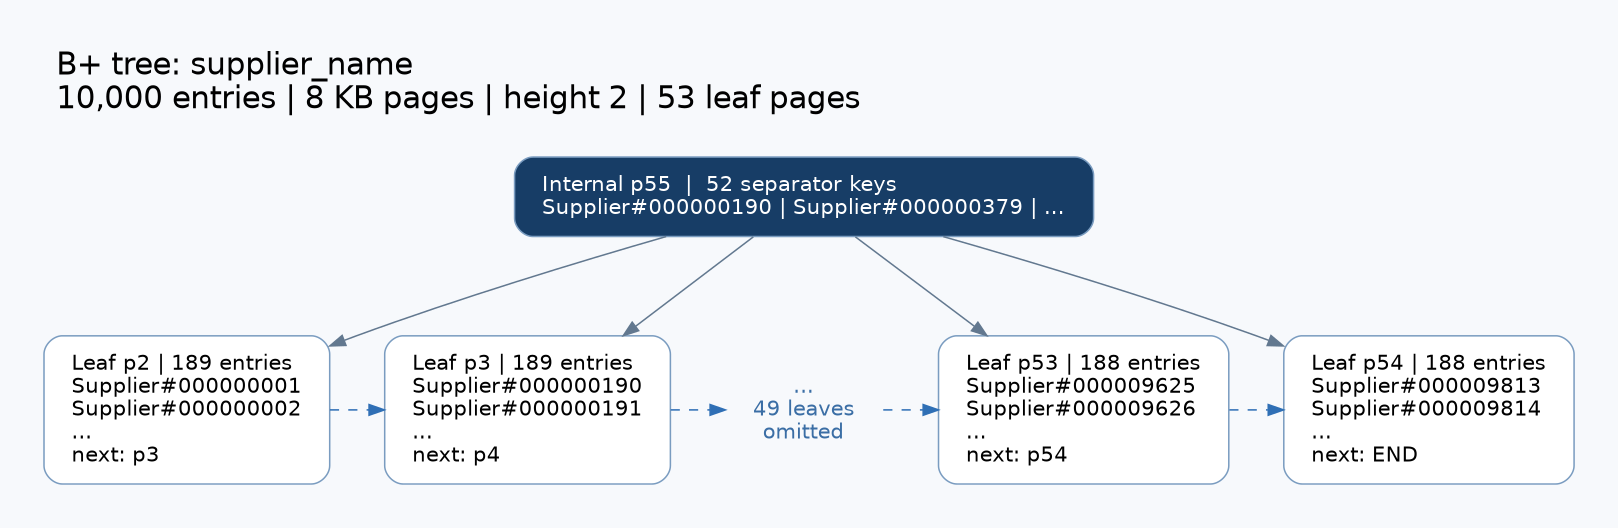
\includegraphics[width=\textwidth]{../exp2-evidence/supplier_name.png}
  \caption{supplier 字符索引的 B+ 树}
  \label{fig:name}
\end{figure}

验收程序的输出：

\begin{lstlisting}[style=wide]
supplier_rows=10000 buffer_frames=16 build_seconds=0.0123916
supplier_key valid=ok entries=10000 height=2 nodes=27 leaves=26 free_pages=0 capacity=450 root=4
supplier_name valid=ok entries=10000 height=2 nodes=54 leaves=53 free_pages=0 capacity=218 root=4
reopen_point_lookups=20000 range_vs_heap=OK insert_update_delete=OK
buffer_miss=1022 evict=1020 flush=36
final_reopen=OK
\end{lstlisting}

关闭并重新打开数据库后，按两种键分别核对全部源记录，共 2 万次点查找全部一致；范围查询与全表扫描结果一致；插入、改键、改名、删除以及再次重开后的核对全部通过。

\subsection{演示脚本输出}

以下是 \code{scripts/demo\_index.txt} 的部分输出（Release 构建，16 帧缓冲池）。

\paragraph{建立索引与命令行树图}两个索引都在内存内排序后建成；\code{index\_tree} 的输出只截取了前几个叶子。
\begin{lstlisting}[style=wide]
CREATE INDEX supplier_key ON supplier(s_suppkey);
CREATE INDEX supplier_key (B+ tree, 10000 entries, sorted in memory)
Run Time: 0.006 s
CREATE INDEX supplier_name ON supplier(s_name);
CREATE INDEX supplier_name (B+ tree, 10000 entries, sorted in memory)
Run Time: 0.007 s
PRAGMA indexes(supplier);
index         | table    | column    | type     | entries
--------------+----------+-----------+----------+--------
supplier_key  | supplier | s_suppkey | INTEGER  | 10000
supplier_name | supplier | s_name    | CHAR(25) | 10000
(2 rows)
Run Time: 0.000 s
PRAGMA index_stats(supplier_key);
valid | entries | height | nodes | leaves | free_pages | capacity | root
------+---------+--------+-------+--------+------------+----------+-----
ok    | 10000   | 2      | 27    | 26     | 0          | 450      | 4
(1 row)
Run Time: 0.000 s
PRAGMA index_stats(supplier_name);
valid | entries | height | nodes | leaves | free_pages | capacity | root
------+---------+--------+-------+--------+------------+----------+-----
ok    | 10000   | 2      | 54    | 53     | 0          | 218      | 4
(1 row)
Run Time: 0.003 s
PRAGMA index_tree(supplier_key);
B+ tree supplier_key (10000 entries)
`-- INTERNAL p4 [25] "386"@73:8 | "771"@81:14 | "1156"@89:20 | "1541"@97:27 | ...
    |-- LEAF p2 [385] "1"@65:0 | "2"@65:1 | "3"@65:2 | "4"@65:3 | ... -> p3
    |-- LEAF p3 [385] "386"@73:8 | "387"@73:9 | "388"@73:10 | "389"@73:11 | ... -> p5
    |-- LEAF p5 [385] "771"@81:14 | "772"@81:15 | "773"@81:16 | "774"@81:17 | ... -> p6
    |-- LEAF p6 [385] "1156"@89:20 | "1157"@89:21 | "1158"@89:22 | "1159"@89:23 | ... -> p7
    ...
\end{lstlisting}

\paragraph{基于索引的查找}两种类型上的等值查找和整型上的范围查找，消息中的 \code{INDEX SCAN} 表示使用了索引。
\begin{lstlisting}[style=wide]
SELECT rid, s_suppkey, s_name FROM supplier WHERE s_suppkey = 42;
rid   | s_suppkey | s_name
------+-----------+-------------------
65:41 | 42        | Supplier#000000042
(1 row)
INDEX SCAN supplier_key
Run Time: 0.000 s
SELECT rid, s_suppkey, s_name FROM supplier WHERE s_name = 'Supplier#000000042';
rid   | s_suppkey | s_name
------+-----------+-------------------
65:41 | 42        | Supplier#000000042
(1 row)
INDEX SCAN supplier_name
Run Time: 0.000 s
SELECT s_suppkey, s_name FROM supplier WHERE s_suppkey >= 9995 LIMIT 6;
s_suppkey | s_name
----------+-------------------
9995      | Supplier#000009995
9996      | Supplier#000009996
9997      | Supplier#000009997
9998      | Supplier#000009998
9999      | Supplier#000009999
10000     | Supplier#000010000
(6 rows)
INDEX SCAN supplier_key
Run Time: 0.000 s
\end{lstlisting}

\paragraph{插入、更新、删除}更新同时修改了两个被索引的列；之后按旧键查不到、按新名字能查到；删除后两个索引都查不到，最后校验两棵树。
\begin{lstlisting}[style=wide]
INSERT INTO supplier VALUES (-1, 'IndexDemo', 'demo address', 0, '00-000-000-0000', 12.34, 'new index entry');
INSERT 1 row(s) into supplier
changes: 1
Run Time: 0.000 s
SELECT rid, s_suppkey, s_name FROM supplier WHERE s_suppkey = -1;
rid    | s_suppkey | s_name
-------+-----------+----------
276:17 | -1        | IndexDemo
(1 row)
INDEX SCAN supplier_key
Run Time: 0.000 s
UPDATE supplier SET s_suppkey = -2, s_name = 'IndexChanged' WHERE s_suppkey = -1;
UPDATE 1 row(s) in supplier
INDEX SCAN supplier_key
changes: 1
Run Time: 0.000 s
SELECT s_suppkey, s_name FROM supplier WHERE s_suppkey = -1;
s_suppkey | s_name
----------+-------
(0 rows)
INDEX SCAN supplier_key
Run Time: 0.000 s
SELECT rid, s_suppkey, s_name FROM supplier WHERE s_name = 'IndexChanged';
rid    | s_suppkey | s_name
-------+-----------+-------------
276:17 | -2        | IndexChanged
(1 row)
INDEX SCAN supplier_name
Run Time: 0.000 s
DELETE FROM supplier WHERE s_suppkey = -2;
DELETE 1 row(s) from supplier
INDEX SCAN supplier_key
changes: 1
Run Time: 0.000 s
SELECT s_suppkey, s_name FROM supplier WHERE s_name = 'IndexChanged';
s_suppkey | s_name
----------+-------
(0 rows)
INDEX SCAN supplier_name
Run Time: 0.000 s
PRAGMA index_check(supplier_key);
valid | entries | height | nodes | leaves | free_pages | capacity | root
------+---------+--------+-------+--------+------------+----------+-----
ok    | 10000   | 2      | 27    | 26     | 0          | 450      | 4
(1 row)
Run Time: 0.000 s
PRAGMA index_check(supplier_name);
valid | entries | height | nodes | leaves | free_pages | capacity | root
------+---------+--------+-------+--------+------------+----------+-----
ok    | 10000   | 2      | 54    | 53     | 0          | 218      | 4
(1 row)
Run Time: 0.003 s
\end{lstlisting}

\paragraph{小内存预算下的外部归并建树与缓冲池统计}把排序预算设为 64 KB，1 万个键放不下，建树过程落盘为 3 个有序段再归并。
\begin{lstlisting}[style=wide]
PRAGMA index_sort_memory = 64;
index_sort_memory_kb
--------------------
64
(1 row)
Run Time: 0.000 s
CREATE INDEX supplier_nation ON supplier(s_nationkey);
CREATE INDEX supplier_nation (B+ tree, 10000 entries, external sort: 3 runs merged in 1 pass)
Run Time: 0.005 s
PRAGMA index_check(supplier_nation);
valid | entries | height | nodes | leaves | free_pages | capacity | root
------+---------+--------+-------+--------+------------+----------+-----
ok    | 10000   | 2      | 27    | 26     | 0          | 450      | 4
(1 row)
Run Time: 0.001 s
SELECT s_suppkey, s_nationkey FROM supplier WHERE s_nationkey = 7 LIMIT 3;
s_suppkey | s_nationkey
----------+------------
33        | 7
44        | 7
53        | 7
(3 rows)
INDEX SCAN supplier_nation
Run Time: 0.000 s
PRAGMA buffer_stats;
frames | used | pinned | dirty | hit   | miss | hit_rate | evict | flush | new_page
-------+------+--------+-------+-------+------+----------+-------+-------+---------
16     | 16   | 0      | 0     | 30399 | 1054 | 96.65    | 1329  | 353   | 353
(1 row)
Run Time: 0.000 s
\end{lstlisting}

\subsection{规模测试}

\paragraph{orders（150 万行）}在 \code{o\_orderkey}、\code{o\_custkey}（\code{INTEGER}）和 \code{o\_clerk}（\code{CHAR(15)}）上建三个索引，默认 8 MB 缓冲池。表~\ref{tab:orders} 同时给出第一版实现（逐条插入建树、节点整页解码、\code{UPDATE/DELETE} 扫描全表）在同一台机器上的结果作为对照。

\begin{table}[H]
  \centering
  \caption{orders 150 万行上的结果}
  \label{tab:orders}
  \begin{tabular}{lrr}
    \toprule
    操作 & 第一版 & 当前版本 \\
    \midrule
    \code{COPY} 导入（无索引） & 约 4 s & 约 4 s \\
    \code{CREATE INDEX}（每个索引） & 41--48 s & 0.6--1.5 s \\
    点查 \code{o\_orderkey = ...}（无索引 0.367 s） & 小于 0.001 s & 小于 0.001 s \\
    按键 \code{UPDATE} / \code{DELETE} 单行 & 约 0.4 s & 小于 0.001 s \\
    范围 \code{DELETE} 约 10 万行，维护三个索引 & 25.8 s & 3.0--3.6 s \\
    先建三个索引再 \code{COPY} 150 万行 & 187 s & 66 s \\
    \bottomrule
  \end{tabular}
\end{table}

三棵树高度都是 3，节点数分别为 3819、3819 和 5727，增删改之后 \code{index\_check} 全部通过。最后一行是逐条维护的路径：剩余的时间主要是 8 MB 缓冲池下随机键插入引起的换页 I/O：只建 \code{o\_custkey} 一个随机键索引时导入需 25.8 s，期间约 69 万次缺页、72 万次写回；把缓冲池调到 128 MB 后降到 10 s。这也直接体现了缓冲池大小对外存索引的影响。

\paragraph{lineitem（600 万行）：外部归并建树}表~\ref{tab:lineitem} 是不同排序内存预算下的建树结果。进程内存峰值用 \code{/usr/bin/time} 测得，包含 8 MB 缓冲池；不建索引时进程本身约 9 MB。

\begin{table}[H]
  \centering
  \caption{lineitem 600 万行上建索引}
  \label{tab:lineitem}
  \begin{tabular}{llrrr}
    \toprule
    索引列 & 排序预算 & 有序段数 & 建树耗时 & 进程内存峰值 \\
    \midrule
    \code{l\_orderkey} INTEGER & 64 MB（默认） & 2 & 3.0--3.6 s & 74 MB \\
    \code{l\_shipinstruct} CHAR(25) & 64 MB（默认） & 3 & 5.3--5.9 s & 71 MB \\
    \code{l\_shipinstruct} CHAR(25) & 8 MB & 20 & 5.4 s & 18 MB \\
    \code{l\_orderkey} INTEGER & 64 KB & 1710（4 趟归并） & 4.6 s & 12 MB \\
    \bottomrule
  \end{tabular}
\end{table}

两棵树高度均为 3（15272 和 31585 个节点），校验通过，之后的索引查找和删除维护正常。内存峰值跟随预算而不是表的大小：预算从 64 MB 降到 64 KB，有序段从 2 个增加到 1710 个，需要 4 趟归并，耗时只增加约一秒。作为对照，开发过程中一个不限内存、全部在内存排序的中间版本在同样的数据上峰值为 600--794 MB。

\subsection{测试中发现的问题}

\begin{itemize}
  \item \textbf{整数比较的精度}：SQL 层原来把数值统一转成 \code{long double} 比较，在 Apple Silicon 上它只有双精度，超过 $2^{53}$ 的相邻 \code{BIGINT} 会被当成相等。改为整数之间直接按 64 位比较，并加入了对应的边界测试。
  \item \textbf{字符串的比较语义}：改为按页内字节比较时，必须保持“尾部空白不参与比较”的语义，否则 \code{CHAR} 列补齐空格的键会与原有顺序不一致。
  \item \textbf{堆扫描路径的 NULL}：把三处重复的过滤逻辑合并成 \code{FindRows} 时，一度漏掉了“\code{NULL} 不满足任何比较”的判断，会使 \code{NULL} 行被 $<$ 条件命中；已修正，并由含 \code{NULL} 的对照测试覆盖。
  \item \textbf{排序缓冲的内存}：外部排序的第一版让缓冲按翻倍增长，实测内存峰值是预算的两倍；改为一次按预算分配、放不下就落盘。归并阶段原来每个有序段固定 64 KB 读缓冲，段数很多时归并内存会超过预算；改为限制归并路数并做多趟归并。
\end{itemize}

% ================================================================== 6
\section{实验总结}

\subsection{完成情况}

\begin{table}[H]
  \centering
  \caption{对照实验要求}
  \begin{tabularx}{\textwidth}{l X}
    \toprule
    要求 & 完成情况 \\
    \midrule
    索引的初始建立 & \code{CREATE INDEX} 对已有数据建树：外部归并排序加自底向上装载 \\
    索引的维护（增、删、改） & 插入与分裂、删除与借位合并、根收缩、空闲页复用；\code{INSERT/COPY/UPDATE/DELETE} 自动维护 \\
    索引的查找 & 等值与范围查找，\code{SELECT/UPDATE/DELETE} 自动使用索引 \\
    外存索引、内外存数据交换 & 节点为磁盘页，全部经缓冲池读写；2 帧缓冲池下可用；建树的排序内存有上限 \\
    两种数据类型 & 整型（\code{INTEGER}、\code{BIGINT}）与字符型（\code{CHAR}、\code{VARCHAR}） \\
    图形化展示 & 命令行树图、Graphviz 图源、由树图生成的结构图 \\
    测试数据规模 & TPC-H supplier 1 万行、orders 150 万行、lineitem 600 万行 \\
    \bottomrule
  \end{tabularx}
\end{table}

\subsection{收获与体会}

\begin{itemize}
  \item \textbf{存储层的接口决定了索引好不好写}。实验一的堆表保证行搬家后 RID 不变，索引里的记录地址因此永远有效，更新不涉及索引列时索引完全不用动。缓冲池的 \code{PageGuard} 和统一的页头、校验和也被索引原样复用。
  \item \textbf{把（键，RID）整体作为排序键}，使重复键、精确删除和分隔键的语义都变得简单，这比为重复键另设溢出页要省事得多。
  \item \textbf{先测量再优化}。第一版功能正确，但建 150 万行的索引要四十多秒。性能分析指出时间花在每次访问节点时的整页解码上，而不是我们最初猜测的元数据页写回或磁盘 I/O；针对它改为按页内字节操作，并用批量建树绕开逐条插入，才得到数量级的改进。
  \item \textbf{对照测试很有效}。让同一批语句在有索引和无索引的表上执行并比较结果，不需要为每种情况手写期望值，就发现了合并过滤逻辑时引入的 \code{NULL} 处理错误。
  \item \textbf{“外存”要落实到每个环节}。树本身按页换入换出还不够，建树时把整列读进内存排序同样会让内存随数据增长；按照成熟系统的做法补上外部归并之后，建索引的内存才真正由配置决定。
\end{itemize}

\subsection{不足与后续工作}

\begin{itemize}
  \item 只支持单列、非唯一索引，不支持复合索引和唯一约束，也不支持在 \code{DATE}、\code{DECIMAL}、\code{FLOAT} 列上建索引。
  \item 字符串键按声明长度定长存储，声明很长而实际很短的 \code{VARCHAR} 列会浪费空间、降低扇出；叶子和内部节点共用一个容量，叶子页有约五分之一的空间用不上。两者都需要修改磁盘格式。
  \item 没有日志和崩溃恢复：正常关闭和重开是有保证的，但索引维护中途崩溃可能使索引与表不一致。目前的处理是维护失败时删除该表的索引，由用户重建。这部分留给后续的故障恢复实验。
  \item 索引通过扫描目录发现，没有登记在系统目录里；排序内存预算只对当前会话有效。
  \item 查询只支持单个比较条件，没有基于代价的访问路径选择（目前的规则是：有索引且不是 $\neq$ 就用）。
\end{itemize}

% ================================================================== 7
\section{核心源代码}

以下代码摘自仓库，注释为源码原文。

\subsection{节点内的比较与二分查找（\code{src/index/bplus\_tree.cpp}）}

\begin{lstlisting}[language=C++]
// Key of slot i against `key`, agreeing with CompareValues.
int CompareKey(size_t i, const Value& key) const {
  const std::byte* slot = Slot(i);
  if (tree_.string_keys_) {
    const int cmp =
        TrimmedRight(StringKey(slot)).compare(TrimmedRight(key.string_value));
    return cmp < 0 ? -1 : cmp > 0 ? 1 : 0;
  }
  const int64_t a = IntegerKey(slot), b = IntegerOf(key);
  return a < b ? -1 : a > b ? 1 : 0;
}
// Slot i against `probe` in (key, RID) order.
int Compare(size_t i, const IndexEntry& probe) const {
  const int key = CompareKey(i, probe.key);
  return key ? key : CompareRids(Rid(Slot(i)), probe.rid);
}
// First slot not less than `probe`: where it is, or belongs, in a leaf.
size_t LowerBound(const IndexEntry& probe) const {
  size_t low = 0, high = size();
  while (low < high) {
    const size_t middle = (low + high) / 2;
    if (Compare(middle, probe) < 0)
      low = middle + 1;
    else
      high = middle;
  }
  return low;
}
// Child to descend into: a separator equal to `probe` sends it right.
size_t ChildIndex(const IndexEntry& probe) const {
  size_t low = 0, high = size();
  while (low < high) {
    const size_t middle = (low + high) / 2;
    if (Compare(middle, probe) <= 0)
      low = middle + 1;
    else
      high = middle;
  }
  return low;
}
\end{lstlisting}

\subsection{节点内的插入与删除（\code{src/index/bplus\_tree.cpp}）}

\begin{lstlisting}[language=C++]
// Inserts `entry` as slot `at`; in an internal node `right_child` becomes
// child at + 1. A full node may take one more slot until it is split.
void Insert(size_t at, const IndexEntry& entry,
            page_id_t right_child = kInvalidPageId) {
  std::byte* slot = Slot(at);
  std::memmove(slot + slot_bytes(), slot, (size() - at) * slot_bytes());
  set_size(size() + 1);
  SetKey(at, entry);
  if (!leaf_) WriteU32(slot, tree_.key_bytes_ + kRidBytes, right_child);
}
void Append(const IndexEntry& entry, page_id_t right_child = kInvalidPageId) {
  Insert(size(), entry, right_child);
}
// Appends slots [from, from + count) of `source`, a node of the same kind.
void Append(const Node& source, size_t from, size_t count) {
  std::memcpy(Slot(size()), source.Slot(from), count * slot_bytes());
  set_size(size() + count);
}
// Replaces the key and RID of slot `at`, keeping its child.
void SetKey(size_t at, const IndexEntry& entry) {
  std::byte* slot = Slot(at);
  if (tree_.string_keys_) {
    const std::string& text = entry.key.string_value;
    std::memset(slot, 0, tree_.key_bytes_);
    WriteU16(slot, 0, static_cast<uint16_t>(text.size()));
    std::memcpy(slot + 2, text.data(), text.size());
  } else {
    const int64_t value = IntegerOf(entry.key);
    std::memcpy(slot, &value, sizeof(value));
  }
  WriteU32(slot, tree_.key_bytes_, entry.rid.page_id);
  WriteU16(slot, tree_.key_bytes_ + 4, entry.rid.slot);
}
// Removes slot `at`: in an internal node, separator at and child at + 1.
void Erase(size_t at) {
  std::byte* slot = Slot(at);
  std::memmove(slot, slot + slot_bytes(), (size() - at - 1) * slot_bytes());
  set_size(size() - 1);
}
\end{lstlisting}

\subsection{插入与分裂（\code{src/index/bplus\_tree.cpp}）}

\begin{lstlisting}[language=C++]
Result<std::optional<BPlusTree::Split>> BPlusTree::InsertNode(
    page_id_t id, const IndexEntry& entry) {
  Node n(*this);
  auto status = Read(id, &n);
  if (!status.ok()) return status;
  if (n.leaf()) {
    const size_t at = n.LowerBound(entry);
    if (at < n.size() && n.Compare(at, entry) == 0)
      return Status(StatusCode::kAlreadyExists, "index entry already exists");
    n.Insert(at, entry);
  } else {
    const size_t at = n.ChildIndex(entry);
    auto split = InsertNode(n.child(at), entry);
    if (!split.ok()) return split.status();
    if (!split.value()) return std::optional<Split>{};
    n.Insert(at, split.value()->separator, split.value()->right);
  }
  if (n.size() <= capacity_) {
    status = Write(n);
    if (!status.ok()) return status;
    return std::optional<Split>{};
  }
  // Split: the upper half moves to a new right sibling. A leaf keeps the
  // separator as the sibling's first entry; an internal node moves it up.
  auto allocated = Allocate();
  if (!allocated.ok()) return allocated.status();
  Node right(*this);
  right.Reset(allocated.value(), n.leaf());
  const size_t middle = n.size() / 2;
  Split split{n.entry(middle), right.id()};
  if (n.leaf()) {
    right.Append(n, middle, n.size() - middle);
    right.set_next(n.next());
    n.set_next(right.id());
  } else {
    right.set_first_child(n.child(middle + 1));
    right.Append(n, middle + 1, n.size() - middle - 1);
  }
  n.Truncate(middle);
  status = Write(right);
  if (!status.ok()) return status;
  status = Write(n);
  if (!status.ok()) return status;
  return std::optional<Split>{split};
}
\end{lstlisting}

\subsection{借位与合并（\code{src/index/bplus\_tree.cpp}）}

\begin{lstlisting}[language=C++]
// Restores the minimum fill of `parent`'s child `at` after an erase left it
// short: borrow one entry from the left sibling, else from the right, else
// merge with a sibling, which takes a separator out of `parent`.
Status BPlusTree::Rebalance(Node* parent, size_t at) {
  const size_t minimum = capacity_ / 2;
  Node child(*this), left(*this), right(*this);
  auto s = Read(parent->child(at), &child);
  if (!s.ok()) return s;
  const bool has_left = at > 0, has_right = at < parent->size();
  if (has_left) {
    s = Read(parent->child(at - 1), &left);
    if (!s.ok()) return s;
    if (left.size() > minimum) {
      const size_t last = left.size() - 1;
      if (child.leaf()) {
        child.Insert(0, left.entry(last));
        parent->SetKey(at - 1, child.entry(0));
      } else {
        // Rotate through the parent: its separator comes down, the left
        // sibling's last separator goes up and its last child moves over.
        child.Insert(0, parent->entry(at - 1), child.child(0));
        child.set_first_child(left.child(last + 1));
        parent->SetKey(at - 1, left.entry(last));
      }
      left.Truncate(last);
      s = Write(left);
      if (!s.ok()) return s;
      return Write(child);
    }
  }
  if (has_right) {
    s = Read(parent->child(at + 1), &right);
    if (!s.ok()) return s;
    if (right.size() > minimum) {
      if (child.leaf()) {
        child.Append(right.entry(0));
        right.Erase(0);
        parent->SetKey(at, right.entry(0));
      } else {
        child.Append(parent->entry(at), right.child(0));
        parent->SetKey(at, right.entry(0));
        right.set_first_child(right.child(1));
        right.Erase(0);
      }
      s = Write(right);
      if (!s.ok()) return s;
      return Write(child);
    }
  }
  // Merge the right node of the pair into the left one.
  Node& into = has_left ? left : child;
  const Node& from = has_left ? child : right;
  const size_t separator = has_left ? at - 1 : at;
  if (into.leaf())
    into.set_next(from.next());
  else
    into.Append(parent->entry(separator), from.child(0));
  into.Append(from, 0, from.size());
  s = Write(into);
  if (!s.ok()) return s;
  s = Free(from.id());
  if (!s.ok()) return s;
  parent->Erase(separator);
  return Status::Ok();
}
\end{lstlisting}

\subsection{删除（\code{src/index/bplus\_tree.cpp}）}

\begin{lstlisting}[language=C++]
// `remaining` receives the number of slots left in node `id`. Only nodes that
// change are written: the leaf, and ancestors whose child had to be rebalanced.
Status BPlusTree::EraseNode(page_id_t id, const IndexEntry& entry,
                            size_t* remaining) {
  Node n(*this);
  auto s = Read(id, &n);
  if (!s.ok()) return s;
  if (n.leaf()) {
    const size_t at = n.LowerBound(entry);
    if (at == n.size() || n.Compare(at, entry) != 0)
      return Status(StatusCode::kNotFound, "index entry not found");
    n.Erase(at);
  } else {
    const size_t at = n.ChildIndex(entry);
    size_t child_size = 0;
    s = EraseNode(n.child(at), entry, &child_size);
    *remaining = n.size();
    if (!s.ok() || child_size >= capacity_ / 2) return s;
    s = Rebalance(&n, at);
    if (!s.ok()) return s;
  }
  *remaining = n.size();
  return Write(n);
}
\end{lstlisting}

\subsection{范围扫描（\code{src/index/bplus\_tree.cpp}）}

\begin{lstlisting}[language=C++]
Status BPlusTree::Scan(CompareOp op, const Value& key,
                       const std::function<bool(const IndexEntry&)>& visitor) {
  if (key.IsNull()) return Status::Ok();  // NULL compares true with nothing
  if (string_keys_
          ? key.kind != ValueKind::kString
          : key.kind != ValueKind::kInt32 && key.kind != ValueKind::kInt64)
    return Status(StatusCode::kTypeMismatch, "wrong index bound type");
  // Operators bounded below start at the key's leaf, the rest at the leftmost
  // leaf; operators bounded above stop at the first entry past the key.
  const bool bounded_below =
      op == CompareOp::kEq || op == CompareOp::kGt || op == CompareOp::kGe;
  const bool bounded_above =
      op == CompareOp::kEq || op == CompareOp::kLt || op == CompareOp::kLe;
  const IndexEntry lowest{key, {0, 0}};
  auto leaf = FindLeaf(bounded_below ? &lowest : nullptr);
  if (!leaf.ok()) return leaf.status();
  Node n(*this);
  for (page_id_t id = leaf.value(); id != kInvalidPageId; id = n.next()) {
    // The copy is not pinned, so the visitor is free to use the buffer pool.
    auto status = Read(id, &n);
    if (!status.ok()) return status;
    for (size_t i = bounded_below ? n.LowerBound(lowest) : 0; i < n.size();
         ++i) {
      const int cmp = n.CompareKey(i, key);
      if (Satisfies(cmp, op)) {
        if (!visitor(n.entry(i))) return Status::Ok();
      } else if (bounded_above && cmp >= 0) {
        return Status::Ok();
      }
    }
  }
  return Status::Ok();
}
\end{lstlisting}

\subsection{多路归并（\code{src/index/bplus\_tree.cpp}）}

\begin{lstlisting}[language=C++]
// The next record in (key, RID) order, valid until the following call;
// null when every run is exhausted.
Status Next(const std::byte** record) {
  if (!started_) {
    started_ = true;
    for (size_t i = 0; i < runs_.size(); ++i) {
      auto status = Push(i);
      if (!status.ok()) return status;
    }
  } else if (!heap_.empty()) {
    // The record handed out last time has been consumed: move its run on.
    std::pop_heap(heap_.begin(), heap_.end(), later_);
    const size_t run = heap_.back();
    heap_.pop_back();
    auto status = Push(run);
    if (!status.ok()) return status;
  }
  *record = heap_.empty() ? nullptr : runs_[heap_.front()].current();
  return Status::Ok();
}
\end{lstlisting}

\subsection{外部排序的收尾：多趟归并与装载（\code{src/index/bplus\_tree.cpp}）}

\begin{lstlisting}[language=C++]
Status BPlusTree::BulkLoader::Finish() {
  if (tree_.entries_ != 0)
    return Status(StatusCode::kInvalidArgument,
                  "bulk load needs an empty tree");
  if (count_ == 0) return Status::Ok();
  if (runs_.empty()) {
    // Everything fit in memory: one sort, no temporary file.
    Sort();
    size_t next = 0;
    return Build([&](const std::byte** record) {
      *record =
          next < offsets_.size() ? arena_.data() + offsets_[next++] : nullptr;
      return Status::Ok();
    });
  }
  if (!offsets_.empty()) {
    auto status = Spill();
    if (!status.ok()) return status;
  }
  arena_ = {};
  offsets_ = {};

  // The budget also bounds the merge: it pays for one read buffer per run, so
  // when there are more runs than buffers, groups of runs are first merged
  // into longer runs until one final merge can feed the build.
  const size_t buffer_bytes = MergeBufferBytes(memory_bytes_);
  const size_t fan_in = std::max<size_t>(memory_bytes_ / buffer_bytes, 2);
  while (runs_.size() > fan_in) {
    auto status = MergePass(fan_in, buffer_bytes);
    if (!status.ok()) return status;
  }
  std::ifstream file(temp_path_, std::ios::binary);
  std::vector<RunReader> readers;
  for (const Run& run : runs_)
    readers.emplace_back(run.offset, run.bytes, buffer_bytes);
  RunMerger merger(file, tree_.string_keys_, std::move(readers));
  return Build([&](const std::byte** record) { return merger.Next(record); });
}
\end{lstlisting}

\subsection{自底向上装载（\code{src/index/bplus\_tree.cpp}）}

\begin{lstlisting}[language=C++]
// Writes the tree bottom-up from the sorted record stream `next`. The entry
// count is known, so the size of every node on every level is planned up
// front and only one node per level is in memory: a leaf fills, is written,
// and hands its page and lowest entry to the level above, which fills the
// same way.
Status BPlusTree::BulkLoader::Build(
    const std::function<Status(const std::byte**)>& next) {
  BPlusTree& tree = tree_;
  // Leave an eighth of each node free so the first inserts do not split.
  const size_t fill = tree.capacity_ - tree.capacity_ / 8;
  struct Level {
    explicit Level(const BPlusTree& tree) : node(tree) {}
    Node node;          // the node being filled
    size_t items = 0;   // entries (leaves) or children (internal) on the level
    size_t nodes = 0;   // nodes the items are spread over
    size_t index = 0;   // which node is being filled
    size_t filled = 0;  // items in it so far
    IndexEntry lowest;  // its lowest entry: the separator its parent stores
    page_id_t reserved = kInvalidPageId;  // page for the next node, if chosen
  };
  std::vector<std::unique_ptr<Level>> levels;
  for (size_t items = count_;; items = levels.back()->nodes) {
    auto level = std::make_unique<Level>(tree);
    level->items = items;
    level->nodes = levels.empty()
                       ? GroupCount(items, fill, tree.capacity_ / 2)
                       : GroupCount(items, fill + 1, tree.capacity_ / 2 + 1);
    levels.push_back(std::move(level));
    if (levels.back()->nodes == 1) break;  // the root
  }
  levels[0]->reserved = tree.root_;  // reuse the empty root page of Create()

  // Puts one item into the node being filled on level `at`; a full node is
  // written and becomes an item of the level above.
  std::function<Status(size_t, const IndexEntry&, page_id_t)> add;
  add = [&](size_t at, const IndexEntry& entry, page_id_t child) -> Status {
    Level& level = *levels[at];
    const bool leaf = at == 0;
    if (level.filled == 0) {
      page_id_t id = level.reserved;
      if (id == kInvalidPageId) {
        auto allocated = tree.Allocate();
        if (!allocated.ok()) return allocated.status();
        id = allocated.value();
      }
      level.reserved = kInvalidPageId;
      level.node.Reset(id, leaf);
      level.lowest = entry;
    }
    if (leaf)
      level.node.Append(entry);
    else if (level.filled == 0)
      level.node.set_first_child(child);
    else
      level.node.Append(entry, child);
    const size_t planned =
        level.items / level.nodes + (level.index < level.items % level.nodes);
    if (++level.filled < planned) return Status::Ok();

    if (leaf && level.index + 1 < level.nodes) {
      // A leaf links to its successor, so that page is chosen now.
      auto allocated = tree.Allocate();
      if (!allocated.ok()) return allocated.status();
      level.reserved = allocated.value();
      level.node.set_next(level.reserved);
    }
    auto status = tree.Write(level.node);
    if (!status.ok()) return status;
    level.filled = 0;
    ++level.index;
    if (at + 1 == levels.size()) {
      tree.root_ = level.node.id();
      return Status::Ok();
    }
    return add(at + 1, level.lowest, level.node.id());
  };

  const bool strings = tree.string_keys_;
  IndexEntry entry;
  entry.key = strings ? Value::String("") : Value::Int64(0);
  std::vector<std::byte> previous;
  uint64_t loaded = 0;
  for (;; ++loaded) {
    const std::byte* record = nullptr;
    auto status = next(&record);
    if (!status.ok()) return status;
    if (!record) break;
    if (!previous.empty() &&
        CompareRecords(strings, previous.data(), record) >= 0)
      return Status(StatusCode::kAlreadyExists, "index entry already exists");
    previous.assign(record, record + RecordBytes(strings, record));
    if (strings)
      entry.key.string_value = RecordString(record);
    else
      entry.key.int64_value = RecordInteger(record);
    entry.rid = RecordRid(strings, record);
    status = add(0, entry, kInvalidPageId);
    if (!status.ok()) return status;
  }
  if (loaded != count_)
    return Status(StatusCode::kInternal, "index sort lost entries");
  tree.entries_ = count_;
  return tree.SaveMetadata();
}
\end{lstlisting}

\subsection{用索引或堆扫描定位行（\code{src/db/database.cpp}）}

\begin{lstlisting}[language=C++]
Result<BPlusTree*> Database::FindRows(const TableInfo& table, Transaction* txn,
                                      const RowFilter& filter,
                                      const RowVisitor& visit) {
  const Schema& schema = table.schema;
  // "<>" matches almost every row: a heap scan beats one random heap read per
  // index entry, so only the other operators use an index.
  BPlusTree* index = filter.column >= 0 && filter.op != CompareOp::kNe
                         ? FindIndex(table, static_cast<size_t>(filter.column))
                         : nullptr;
  if (index) {
    Status row_status;
    const Status status =
        index->Scan(filter.op, filter.value, [&](const IndexEntry& entry) {
          auto tuple = table.heap->Get(txn, entry.rid);
          if (!tuple.ok()) {
            row_status = tuple.status();
            return false;
          }
          auto values = Tuple::Decode(schema, tuple.value().data().data(),
                                      tuple.value().size());
          if (!values.ok()) {
            row_status = values.status();
            return false;
          }
          return visit(entry.rid, tuple.value(), values.value());
        });
    if (!status.ok()) return status;
    if (!row_status.ok()) return row_status;
    return index;
  }

  auto iterator = table.heap->Scan(txn);
  RID rid;
  Tuple tuple;
  while (iterator.Next(&rid, &tuple)) {
    auto values = Tuple::Decode(schema, tuple.data().data(), tuple.size());
    if (!values.ok()) return values.status();
    if (filter.column >= 0) {
      // A NULL column value satisfies no comparison.
      const Value& value = values.value()[filter.column];
      if (value.IsNull() ||
          !Satisfies(CompareValues(value, filter.value), filter.op)) {
        continue;
      }
    }
    if (!visit(rid, tuple, values.value())) break;
  }
  if (!iterator.status().ok()) return iterator.status();
  return static_cast<BPlusTree*>(nullptr);
}
\end{lstlisting}

\end{document}
